\section{Results}


\subsection {Math Cheat Sheet}
\begin{figure}
\begin{center}
    \begin{tikzpicture}
        \begin{axis}
            \addplot[color=red]{exp(x)};
        \end{axis}
    \end{tikzpicture}
    \caption{Plot of Exponential Function.}
    \label{fig:func1} % label must follow caption
\end{center}
\end{figure}



\hskip 5pt

\begin{figure}
\begin{center}
    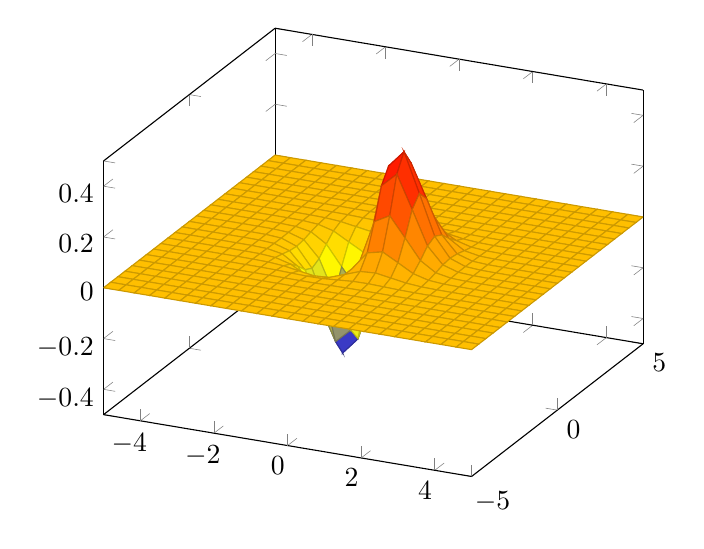
\begin{tikzpicture}
        \begin{axis}
            \addplot3[
                surf,
            ]
            {exp(-x^2-y^2)*x};
        \end{axis}
    \end{tikzpicture}
    \caption{Plot of 3-D Function.}
    \label{fig:func2}
\end{center}
\end{figure}

\begin{figure} [h!] 
    \centering
        \begin{tikzpicture}
        \centering
        \begin{axis}[
            axis lines = left,
            xlabel = $x$,
            ylabel = {$f(x)$},
        ]
        %Below the red parabola is defined
        \addplot [
            domain=-1:1, 
            samples=100, 
            color=red,
        ]
        {e^x};
        \addlegendentry{$e^x$}
        %Here the blue parabola is defined
        \addplot [
            domain=-1:1, 
            samples=100, 
            color=blue,
            ]
            {1/x^2}; % note that the syntax here is different
        \addlegendentry{$\frac{1}{x^2}$}
        \end{axis}
        \end{tikzpicture}
        \caption{Two functions in one plot.}
        \label{fig:func3}
\end{figure}

\autoref{fig:func1}, \autoref{fig:func2}, and \autoref{fig:func3} are generated from function in \LaTeX. 


\subsection{Table Cheat Sheet}

\begin{table}[h]
    \centering
    \begin{tabular}{c|ccc}
        & Apple & Oranges & Strawberries \\
    \hline
    A & 1 & 2 & 3\\
    B & 1 & 2 & 3\\
    C & 1 & 2 & 3\\
    D & 1 & 2 & 3\\
    \end{tabular}
    \caption{Caption}
    \label{tab:my_label}
\end{table}
